\documentclass[english]{SPFShortReport}
\usepackage{subfigure}
\usepackage{longtable}
\usepackage[utf8]{inputenc}
\usepackage{url}
\usepackage{adjustbox}
\usepackage{gensymb}
\usepackage{booktabs}
\usepackage[yyyymmdd,hhmmss]{datetime}
\reportName{System6\_SolarIce\_MFH30\_flatPlate\_HP20-CHE\_tmy-Ac50-Vice20}
\reportSubName{Energy generation costs} 
\reportDate{\today \hspace{0.1cm} at: \currenttime \hspace{0.1cm} h} 
\author{damian.birchler}
\address{damian.birchler}
\begin{document}
\begin{table}[!ht]
\centering
\caption{Assumptions for calculation of heat generation costs}
\begin{adjustbox}{max width =\textwidth}
\begin{tabular}{l | c c c } 
\hline
\hline
$$ &$$ &$$ &$$ \\ 
\hline
Rate & 3.0 \% per annum\\
Analysis period & 30 years\\
Maintenance & 1.0 \% of Investment costs per year \\
\hline \\
Electricity & Fix costs:  0  Fr. per year \\
 & Variable costs:  0.20 $Fr.$ $per$ $kWh$ \\
Increase of electricity costs & 0.0 \% per year \\
Electricity costs year 1 & 4238 Fr. in year 1 \\
Energy demand per year & 49292 kWh \\
\hline
\hline
\end{tabular}
\end{adjustbox}
\label{definitionTable}
\end{table}
\begin{table}[!ht]
\centering
\caption{System and Heat generation costs (all values incl. 8$\%$ VAT) }
\begin{adjustbox}{max width =\textwidth}
\begin{tabular}{l | c c c c c } 
\hline
\hline
Group &Component &Costs &Size &LifeTime &Total Costs \\ 
 & &[CHF] & &Years &[CHF]\\ 
\hline
\\
\textbf{TES} & Storage (Stainless Steel) & -2000+10173$^{\mathrm{+250}}_{\mathrm{-100}}$/m$^3$ & 2.00 m$^3$ & 30 & 18345.6$^{\mathrm{+500.0}}_{\mathrm{-200.0}}$ (13.6$^{\mathrm{+0.9}}_{\mathrm{-1.3}}$\%) \\
 & Storage (Steel) & 666+1214$^{\mathrm{+0}}_{\mathrm{-100}}$/m$^3$ & 1.00 m$^3$ & 30 & 1879.8$^{\mathrm{+0}}_{\mathrm{-100.0}}$ (1.4$^{\mathrm{+0.1}}_{\mathrm{-0.2}}$\%) \\
 & electric rod & 600+0/m$^3$ & 2.00 m$^3$ & 30 & 600.0 (0.4$^{\mathrm{+0.0}}_{\mathrm{-0.0}}$\%) \\
&\cline{1-5}
 & \textbf{Total TES} & & & & 20825.4$^{\mathrm{+500.0}}_{\mathrm{-300.0}}$ (15.5$^{\mathrm{+1.0}}_{\mathrm{-1.6}}$\%) \\
\hline \\
\textbf{Col} & Collector & 9282+875$^{\mathrm{+250}}_{\mathrm{-100}}$/m$^2$ & 50.00 m$^2$ & 30 & 53032.0$^{\mathrm{+12500.0}}_{\mathrm{-5000.0}}$ (39.4$^{\mathrm{+11.3}}_{\mathrm{-6.8}}$\%) \\
\hline \\
\textbf{IceStorage} & Ice Storage (inc. installation) & 0+850/m$^3$ & 20.00 m$^3$ & 20 & 17000.0 (12.6$^{\mathrm{+0.5}}_{\mathrm{-1.1}}$\%) \\
\hline \\
\textbf{Hp} & HeatPump & 8194+363/kW & 20.00 kW & 20 & 15454.0 (11.5$^{\mathrm{+0.5}}_{\mathrm{-1.0}}$\%) \\
\hline \\
\textbf{Installation system} & Installation System (Hydraulics) & 24596+193/kW & 20.00 kW & 30 & 28456.0 (21.1$^{\mathrm{+0.9}}_{\mathrm{-1.9}}$\%) \\
\hline \\
 & \textbf{Total Investment Cost} & & & & \textbf{134767.40$^{\mathrm{+13000.00}}_{\mathrm{-5300.00}}$} (100\%) \\ 
\hline \\ 
\hline \\ 
Annuity & Annuity (yearly costs over lifetime)  &&& & 12987$^{\mathrm{+793}}_{\mathrm{-323}}$ /a  \\
 & Share of Investment & &&& 7401$^{\mathrm{+663}}_{\mathrm{-270}}$ /a (57$^{\mathrm{+ 7}}_{\mathrm{- 5}}$\%) \\
 & Share of Electricity & 0+0.20/kWh & 21190 kWh &  & 4238 /a (33$^{\mathrm{+ 1}}_{\mathrm{- 2}}$\%)\\
 & Share of Maintenance & &&& 1348$^{\mathrm{+130}}_{\mathrm{-53}}$ /a (10$^{\mathrm{+ 1}}_{\mathrm{- 1}}$\%)\\ 
 & Share of Transmission grid & 50+50.00/kWh & 0 kWh & &  0 /a ( 0\%)\\
 & Share of Residual Value &&& &  0 /a ( 0\%)\\
Present Value  & Present Value of all costs  & &&& 244249.14$^{\mathrm{+15548.06}}_{\mathrm{-6338.82}}$ CHF \\
\hline \\ 
 Energy Generation Costs & Using annuity: &&& 26.35$^{\mathrm{+1.61}}_{\mathrm{-0.66}}$ & Rp./kWh \\
\hline
\hline
\end{tabular}
\end{adjustbox}
\label{CostsTable}
\end{table}
\begin{figure}[!htbp]
\begin{center}
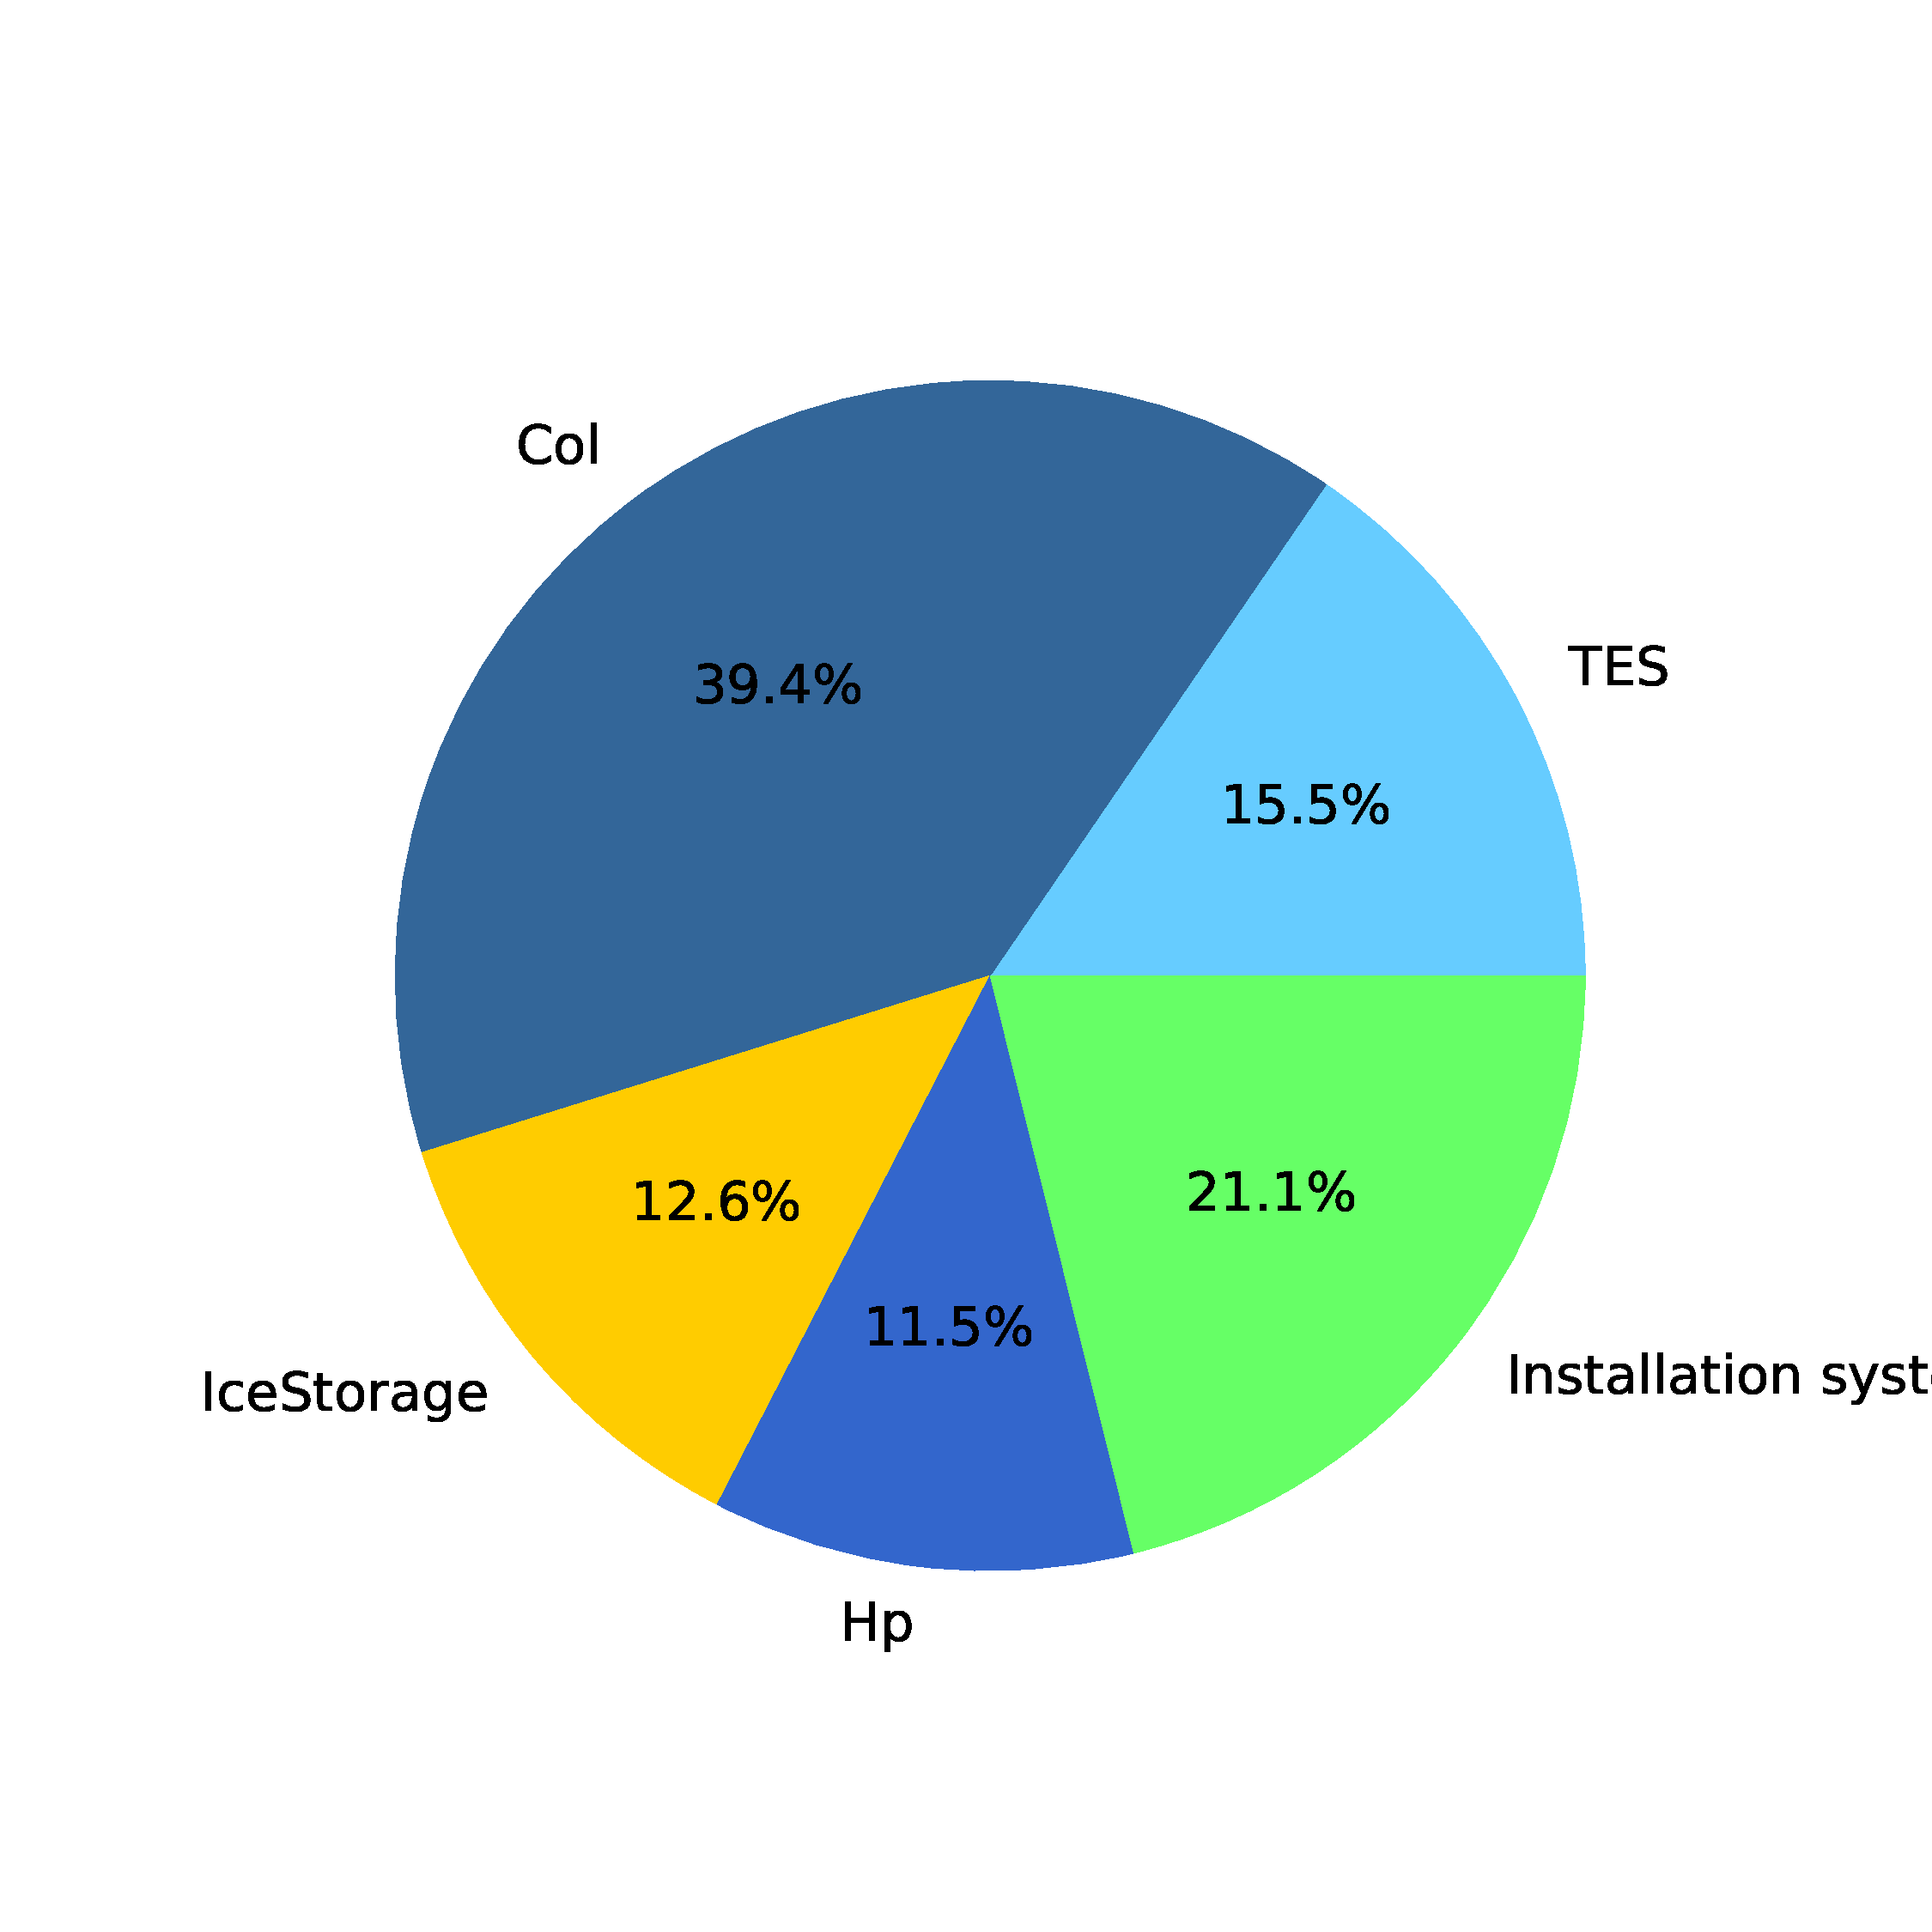
\includegraphics[width=1\textwidth]{costShare-System6_SolarIce_MFH30_flatPlate_HP20-CHE_tmy-Ac50-Vice20.pdf}
\caption{System cost}
\label{systemCost}
\end{center}
\end{figure}
\begin{figure}[!htbp]
\begin{center}
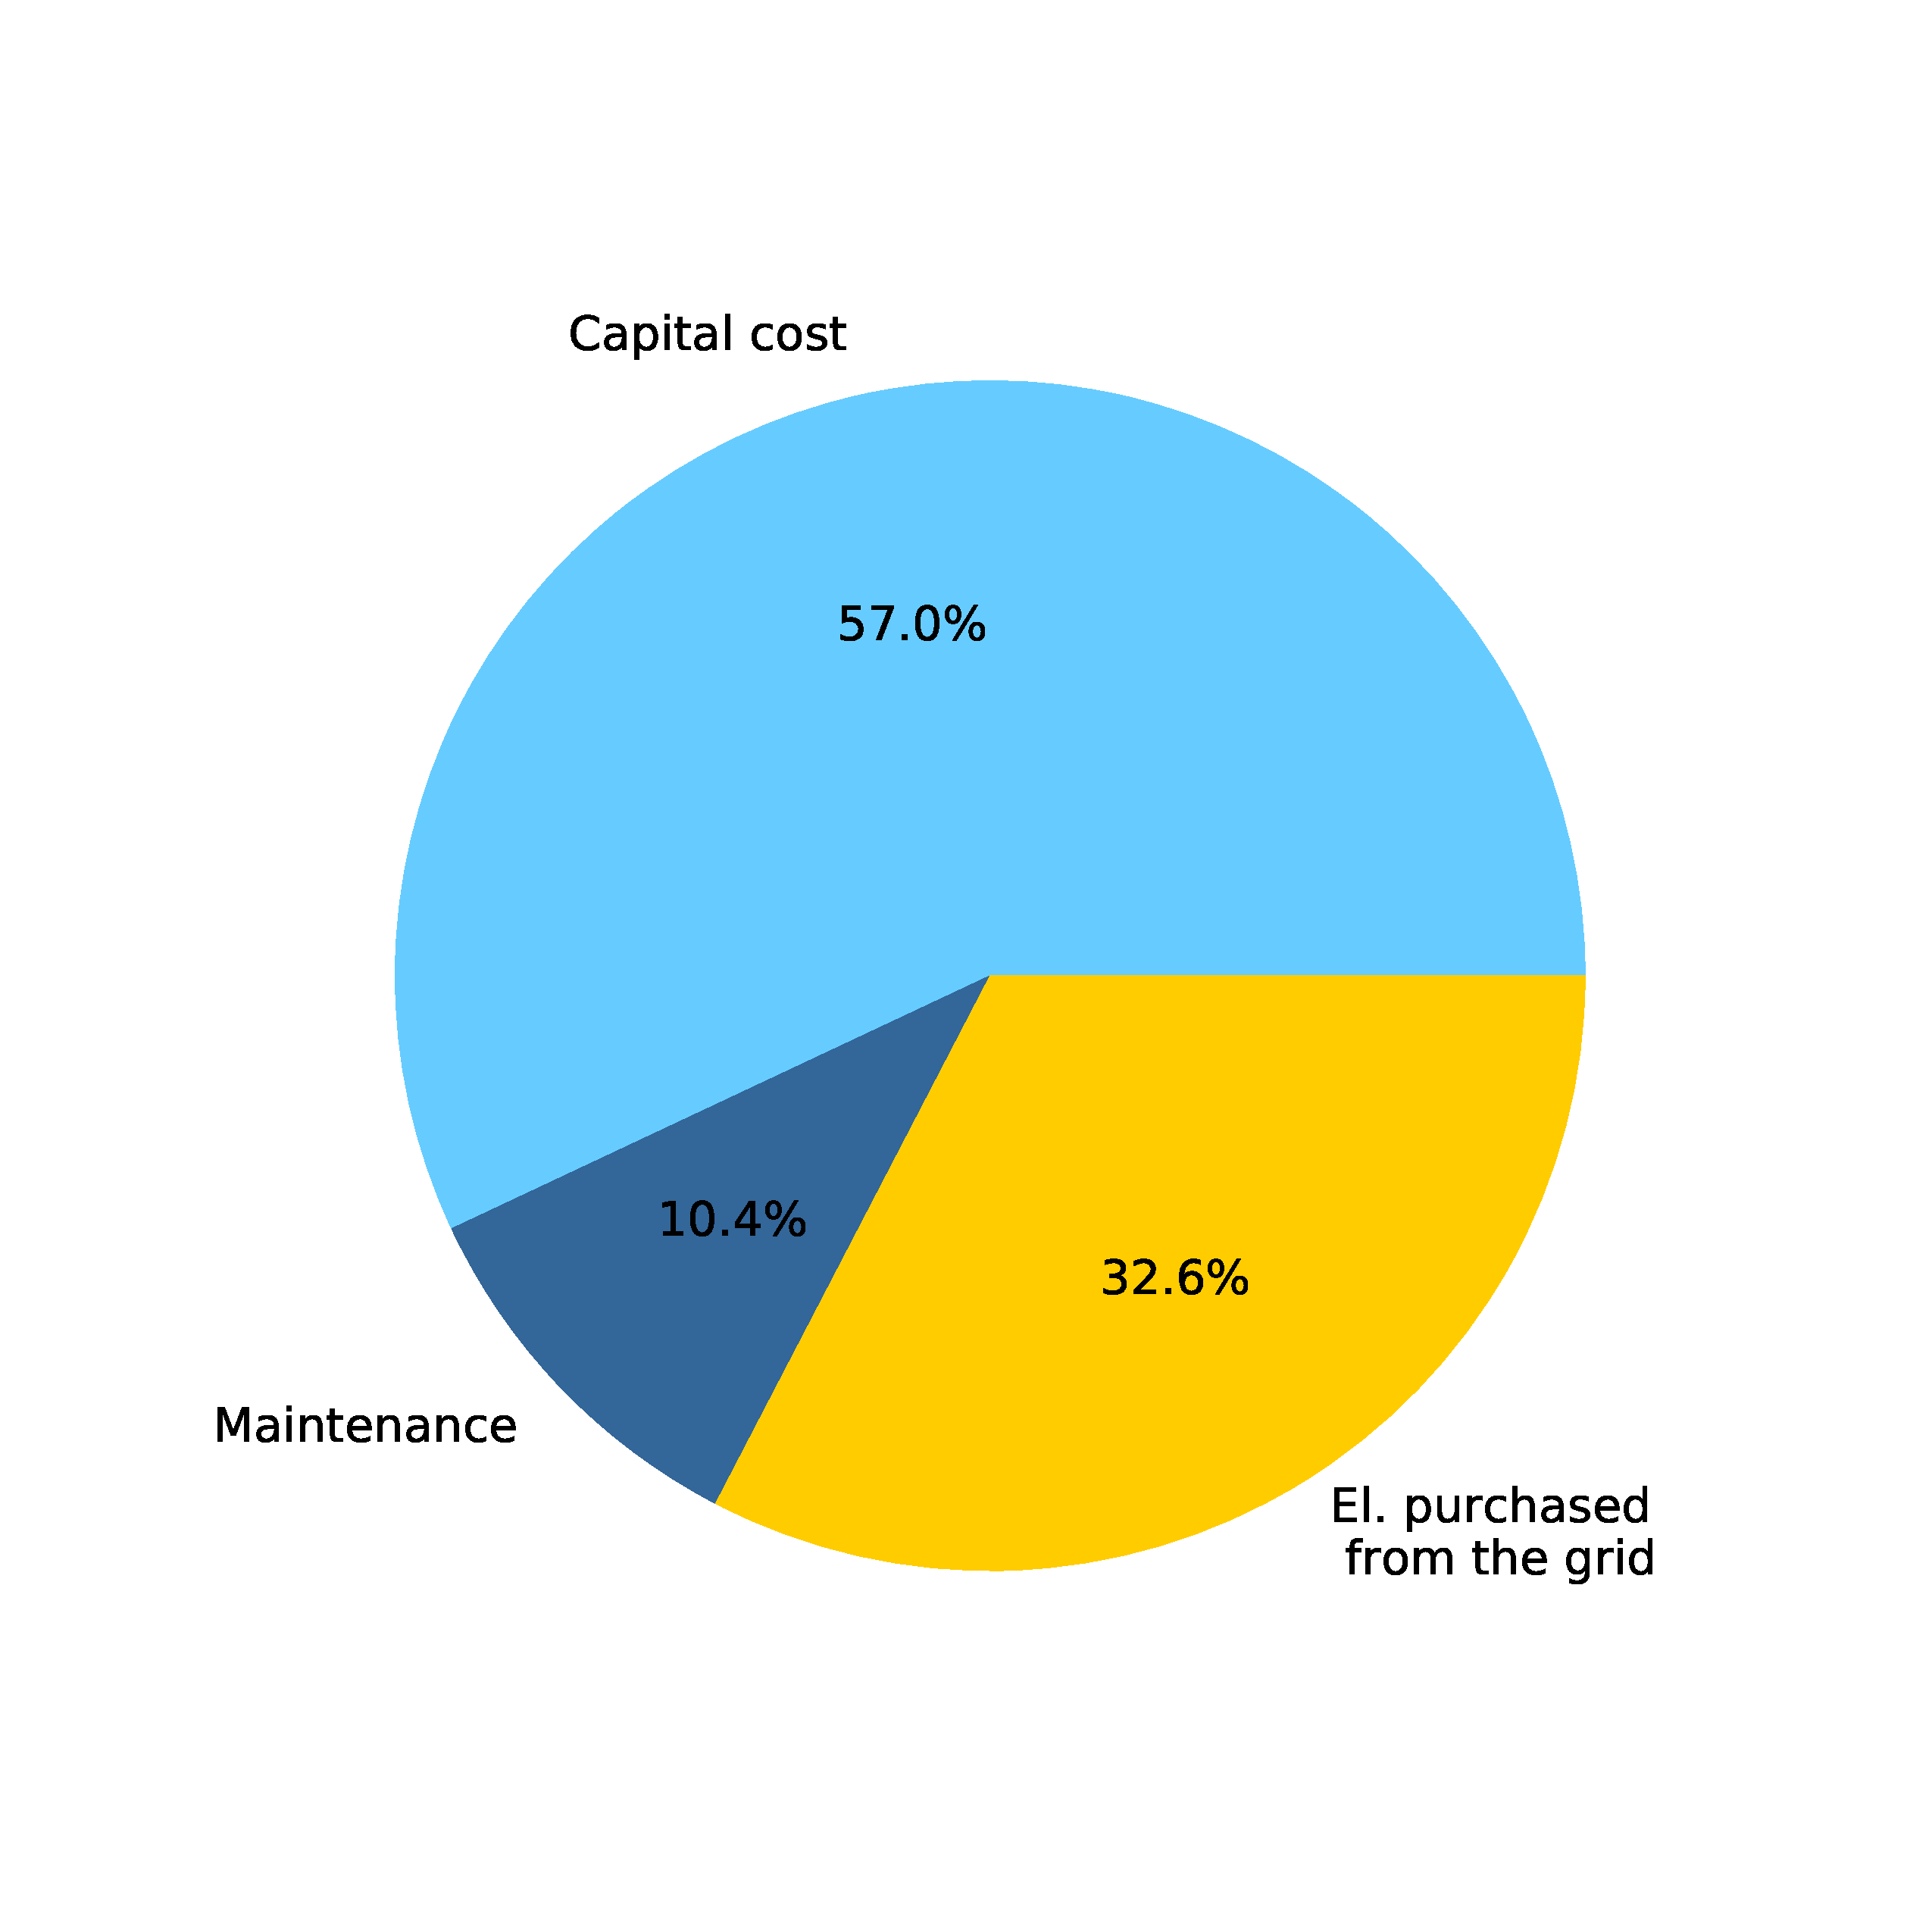
\includegraphics[width=1\textwidth]{costShareAnnuity-System6_SolarIce_MFH30_flatPlate_HP20-CHE_tmy-Ac50-Vice20.pdf}
\caption{System cost annuity share}
\label{systemCostannuity}
\end{center}
\end{figure}
\end{document}
